\section{$\Delta$QSD implementation}

Originally, $\Delta$Q(x) denotes the probability that an outcome occurs in a time $t \le x$, defining then the "intangible mass" of such IRV as $1 - \lim_{x\to\infty} \Delta Q (x)$.
We then extend the original definition to fit real time constraints, needing to calculate $\Delta$Qs continuously.

For a given probe, $\Delta$Q($t_l$, $t_u$, $dMax$) is the probability that the time of series with samples between time $t_l < t_u$, an outcome or probe occurs in time t $\le$ dMax.

\subsection{Internal representation of a $\Delta$Q}
    We provide a $\Delta$Q class to calculate the $\Delta$Q of a probe between a lower time bound $t_l$ and an upper time bound $t_u$.
    
    The $\Delta$Q can be calculated in various ways: 
    
    \paragraph{Observed $\Delta$Q}
    
    The first way is by having $n$ collected outcome instances between $t_l$ and $t_u$, calculating its PDF and then calculating the \textit{empirical cumulative distribution function} (ECDF) based on its PDF. This is called the \textbf{Observed $\Delta$Q}.
    
    \paragraph{Calculated $\Delta$Q}
    
    A $\Delta$Q can also be calculated by performing operations which are the result of outcome expressions on two or more $\Delta$Qs, the notion of outcome instances is then lost between calculations, as the interest shifts towards calculating the resulting PDFs and ECDFs. This is called the \textbf{Calculated $\Delta$Q}.
    
    \subsection{dMax}
        The key concept of $\Delta$QSD is having a maximum delay after which we consider that the execution is failed, this is represented in a prove as $dMax$. The user defines, for each prove the maximum delay its execution can have.

Setting a maximum delay for an prove is not a job that can be done one-off and blindly, it is something that is done with an underlying knowledge of the system inner-workings and must be thoroughly fine tuned during the execution of the system by observing the resulting distributions of the obtained $\Delta$Qs. 

We define in our oscilloscope a formula to dynamically define a maximum delay:
\begin{equation}
    dMax = \Delta_{T} * N  
    \label{eq:dMaxU}
\end{equation}
Where:
\begin{itemize}
    \item $\Delta_{t base}$ represents the base width of a bin, equal to 1ms.
    \item $N$ the number of bins.
\end{itemize}

The user must choose:
\begin{itemize}
    \item $\Delta_T$: $\Delta_T$ is a value which can be set via a slider on the dashboard to control the delay of a probe. 
    \item $N$: We define a range $\lbrack 1, 1000 \rbrack$ for $N$. This is a good enough bound to allow for finer grained bins, or less precision if needed. 
\end{itemize}

Some tradeoffs must though be acknowledged when setting these parameters, a higher number of bins corresponds to a higher number of calculations and space complexity, a lower $dMax$ may correspond to more failures. These are all tradeoffs that must be considered by the system engineer and set accordingly.
    \begin{figure}[H]
        \begin{center}
            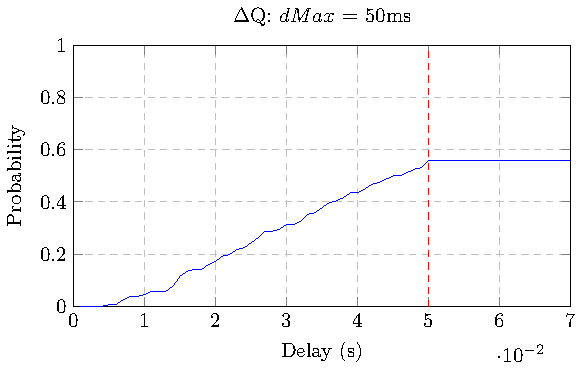
\includegraphics[scale = 1.2]{tikz/cdf_dmax.pdf}
        \end{center}
        \caption{$\Delta$Q: $dMax$ = 50ms, the CDF will stay constant when delay $> dMax$}
    \end{figure}

    \subsection{QTA}
        A simplified QTA is defined for probes. We define 4 points for the step function at 25, 50, 75 percentiles and the maximum amount of failures accepted for an observable. An observed $\Delta$Q will calculate that based on the samples collected. 

    \subsection{Operations}
    In a previous section we talked about the possible operations that can be performed on and between $\Delta$Qs, the time complexity of FTF, ATF and PC is trivially $\mathcal{O}(N)$ where N is the number of bins. As to convolution, the naïve way of calculating convolution has a time complexity of $\mathcal{O}(N^2)$, this quickly becomes a problem as soon as the user wants to have a more fine-grained understanding of a component. Below we present two ways to perform convolution.

        \subsubsection{Convolution} 
            Convolution allows calculating the sum of delays of two causally linked $\Delta$Q$_A$ and $\Delta$Q$_B$. 
        \begin{figure}[H]
            \begin{center}
                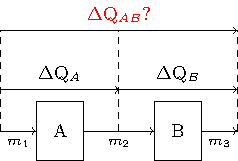
\includegraphics{tikz/comb_dq_comp.pdf}
            \end{center}
        \end{figure}

\subsubsection{Arithmetical operations}
        We can apply a set of arithmetical operations between $\Delta$Qs ECDFs, and on a $\Delta$Q.
    \paragraph{Scaling (multiplication)} A $\Delta$Q can be scaled w.r.t a constant $0 \le j \le 1$. It is equal to binwise multiplication on ECDF bins.
    \begin{equation}
        \hat{f_r}(i) = \hat{f}(i) \cdot j
        \label{eq:mul_ecdf}
    \end{equation}

    \paragraph{Operations between $\Delta$Qs} 
        Addition, subtraction and multiplication can be done between two $\Delta$Q of equal bin width (but not forcibly of equal length) by calculating the operation between the two ECDFs of the $\Delta$Qs:
        \begin{equation}
            \Delta \text{Q}_{AB}(i) = \hat{f_A}(i) [\cdot, +, -] \hat{f_B}(i)
            \label{eq:op_dq}
        \end{equation}
    \subsection{Confidence bounds}
    To observe the stationarity of a system we must observe a window of $\Delta$Qs of an observable and calculate confidence bounds over said windows. The bounds can be updated dynamically by inserting or removing a $\Delta$Q, this allows us to consider a small window of execution rather than observing the whole execution.
        \begin{figure}[H]
            \begin{center}
                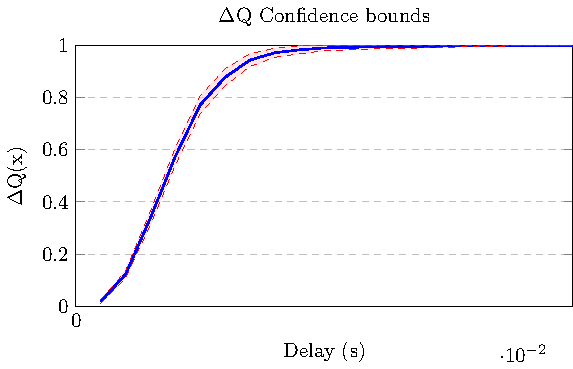
\includegraphics[scale=1.2]{tikz/ci.pdf} 
            \end{center}
            \caption{Upper and lower bounds (dashed, red) of the mean (blue) of multiple $\Delta$Qs. In a system that behaves linearly, the bounds will be close to the mean, once the overload is approaching, or a system is showing behaviour that diverges from a linear one, the bounds will be larger.}
        \end{figure}

  
